\documentclass[crop=false, class=book]{standalone}

%impostazioni lingua
\usepackage[T1]{fontenc}
\usepackage[utf8]{inputenc}
\usepackage[english,italian]{babel}

%sistema i margini
\usepackage{geometry}
\geometry{a4paper,top=2.2cm,bottom=2.2cm,left=3cm,right=3cm, heightrounded}

%interlinea 1.5
\usepackage{setspace}
\onehalfspacing

%gestione delle testatine
\usepackage{fancyhdr}
\pagestyle{fancy}
\lhead{}
\chead{}
\rhead{Titolo}
\lfoot{}
\cfoot{\thepage}
\rfoot{}
\renewcommand{\headrulewidth}{0.4pt}

%formattazione titoli paragrafo
\usepackage{titlesec}
\titleformat{\chapter}[block]{\normalfont\huge\bfseries}{\thechapter.}{0.7em}{\huge}

%pacchetti per i riferimenti in bibliografia
\usepackage[autostyle,italian=guillemets]{csquotes}
\usepackage[style=numeric,citestyle=numeric-comp,backend=biber]{biblatex}

%risorsa che contiene la bibliografia
\addbibresource{./../bibliografia.bib}

\usepackage{lipsum}
\usepackage{graphicx}
\usepackage[italian]{varioref}
\usepackage{copyrightbox}

\begin{document}
		
	\chapter{Depth understanding}
	
		ARCore Depth API  permette agli sviluppatori di generare mappe di profondità attraverso l'uso di algoritmi di 					profondità del movimento. Una mappa di profondità offre una visualizzazione in 3D del mondo reale, ogni pixel è 				associato alla distanza dalla scena e attraverso l'uso di colori differenti è possibile riconoscere quali aree dello 			spazio sono più vicine al dispositivo. Quando viene avviata una nuova sessione ARCore il display dello smartphone è 			nero, ma non appena si effettua un piccolo movimento la profondità viene rilevata. La stima della profondità è ricavata 		attraverso il movimento dello smartphone. Quando si progettano delle applicazioni che si concentrano sulla profondità 			bisogna considerare che la profondità viene calcolata meglio quando la scena rimane la stessa con piccoli spostamenti. 			Il dispositivo ha bisogno di muoversi un pò per generare la profondità. Un altro fattore da prendere in considerazione 			è quando l'utente compie lunghi spostamenti; in questo caso la stima della profondità arriva fino a 8 metri ma la 				migliore accuratezza si ha tra 0 e 5 metri.\\
		 Le principale funzionalità offerte da depth API sono tre:
		
		\begin{itemize}
			\item[•] \textbf{Copertura dei contenuti}: permette di posizionare accuratamente dei contenuti virtuali di fronte o dietro degli oggetti reali.
			\item[•] \textbf{Immersione}: permette di decorare una scena con oggetti virtuali che interagiscono tra di loro.
			\item[•] \textbf{Interazione}: i contenuti virtuali sono in grado di interagire con il mondo reale attraverso cambiamenti fisici e collisioni.
		\end{itemize}
		
		\section{Sessione ARCore con depth API}
		
		Prima di iniziare una nuova sessione ARCore è necessario controllare se il dispositivo supporta depth API. A volte 				questa opzione può essere disattivata oppure non supportata nonostante il dispositivo supporti ARCore. Dopo aver 				definito la sessione con le opportune configurazioni è possibile controllare se il dispositivo e la fotocamera 					supportano una determinata modalità di profondità invocando il metodo \textit{isDepthModeSupported(Config.DepthMode 			mode)} sull'istanza della sessione. Se la modalità è supportata viene configurata la sessione e sarà possibile 					sfruttare depth API.\\ \vref{fig: Controllo supporto depth API}\\
		\clearpage
		\begin{figure}
			\centering
			\copyrightbox[0.5]{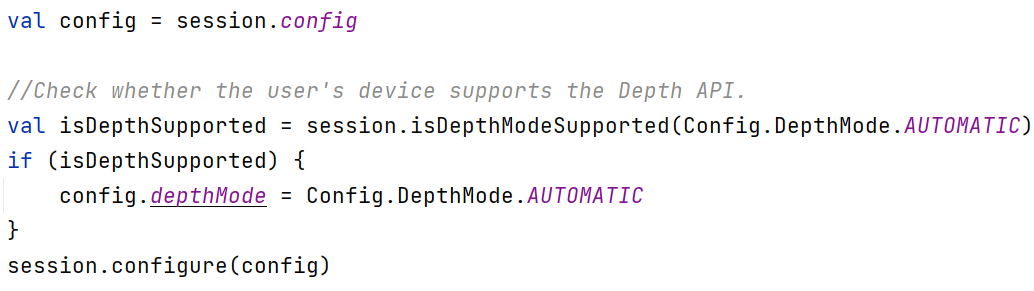
\includegraphics[width=0.8\textwidth]{../../resources/images/depthAPI1.PNG}}%
			{Fonte: \url{https://developers.google.com/ar/develop/java/depth/developer-guide}}
			\caption{Controllo supporto depth API}
			\label{fig: Controllo supporto depth API}
		\end{figure}
		
\end{document}